\documentclass[a4paper, 12pt]{article}
\usepackage{matnoble-doc-en}


\begin{document}

\title{\bf {CHEM400/740: Quantum Mechanics in Chemistry\\ Chapter\#04: Slater Rules and Examples}} \author{\bf
  \href{http://scienide2.uwaterloo.ca/~nooijen/website_new_20_10_2011/About.html}{Marcel Nooijen}} \date{}
  
\pagestyle{fancy} \fancyhead[L]{\textcolor{PrimaryColor}{CHEM400/740: Quantum Mechanics in Chemistry}} \fancyhead[R]{\textcolor{PrimaryColor}{2021 Winter}}


\maketitle
\tableofcontents

\clearpage


\section{Evaluating Matrix Elements Over Slater Determinants}

Formulation of the problem: \\
\tab Given a set of orthonormal spin-orbitals, $\psi_a,\psi_b,...,\psi_m$, we can construct determinants.\\ 
\tab e.g: $|\psi_a\psi_b\psi_c\psi_d| = -|\psi_a\psi_b\psi_d\psi_c| =+|\psi_a\psi_d\psi_b\psi_c|=|K\rangle$\\
\tab We want to evaluate $\langle K|L \rangle$ and $\langle K|\hat{H}|L \rangle=\langle K|\hat{h}|L \rangle + \langle K|\hat{V}|L \rangle$. \\
\tab Note that $\hat{H}=\sum_i\hat{h}(i)+ \sum_{i<j}\frac{1}{r_{ij}}$ and $\hat{h}(i)=\hat{T}_{(i)}+\hat{V}_{(i)}^{Ne}$.\\
\tab We will use antisymmetrizer $\hat{A}$ to define the determinant.
\begin{IEEEeqnarray}{rLl}
\hat{A} &= \frac{1}{N!}\sum_{k=1}^{N!}(-)^{P_k}\hat{P}_k \\
\hat{A}^\dagger &=\hat{A} \\
\hat{A}\hat{A}=N!\hat{A}&=\hat{A}^\dagger\hat{A}=N!\hat{A}^\dagger
\end{IEEEeqnarray}
\tab Normalized basis states:
\begin{IEEEeqnarray}{rLl}
|K\rangle = \frac{1}{\sqrt{N!}}\hat{A}(\psi_a(1)\psi_b(2)\cdots\psi_z(N) )
\end{IEEEeqnarray}
\tab Let us prove this, $\langle K|K\rangle =1$: 
\begin{IEEEeqnarray}{rLl}
\langle K|K\rangle &= \frac{1}{\sqrt{N!}}\frac{1}{\sqrt{N!}}\langle \hat{A}\psi_a(1)\cdots\psi_z(N)|\hat{A}(\psi_a(1)\cdots\psi_z(N)\rangle \notag \\
&= \frac{1}{N!}\langle \psi_a(1)\cdots\psi_z(N)|\hat{A}^\dagger\hat{A}(\psi_a(1)\cdots\psi_z(N))\rangle  \notag \\
&= \frac{1}{N!} N!\langle \psi_a(1)\cdots\psi_z(N)|\hat{A}^\dagger( \psi_a(1)\cdots\psi_z(N))\rangle \notag \\
&= 1 \cdot \langle\hat{A}( \psi_a(1)\cdots\psi_z(N))| \psi_a(1)\cdots\psi_z(N)\rangle \notag \\
&= \int \sum_i (-)^{P_i}\hat{P}_i(\psi_a^*(1)\cdots\psi_z^*(N))\cdot(\psi_a(1)\cdots\psi_z(N)) d1d2\cdots dN  \notag \\
&= \int \psi_a^*(1)\psi_b^*(2)\cdots\psi_z^*(N) \cdot \psi_a(1)\psi_b(2)\cdots\psi_z(N) d\tau \notag \\
&- \int \psi_b^*(1)\psi_a^*(2)\cdots\psi_z^*(N) \cdot \psi_a(1)\psi_b(2)\cdots\psi_z(N) d\tau +\cdots+ \notag \\
&(-)\int \psi_c^*(1)\psi_b^*(2)\cdots\psi_a^*(N) \cdots \psi_a(1)\psi_b(2)\cdots\psi_z(N) d\tau \notag \\
&= 1
\end{IEEEeqnarray}
\tab NOTE:
\begin{itemize}
	\item (|ket$\rangle)^\dagger \Longrightarrow \langle$bra|. e.g: $(\hat{A}|\psi_a\cdots\psi_b\rangle)^\dagger = \langle \psi_a\cdots\psi_b |\hat{A}^\dagger$  \\
	\item Only the identity peremutation contributes; otherwise mismatch. \\
	 $\int \psi_a^*(1)\psi_b^*(2)\cdots\psi_z^*(N) \cdot \psi_a(1)\psi_b(2)\cdots\psi_z(N) d\tau = \langle a|a\rangle_1 \langle b|b\rangle_2 \cdots \langle z|z\rangle_N =1$.\\
	 $\int \psi_b^*(1)\psi_a^*(2)\cdots\psi_z^*(N) \cdot \psi_a(1)\psi_b(2)\cdots\psi_z(N) d\tau =\langle b|a\rangle_1 \langle a|b\rangle_2 \cdots \langle z|z\rangle_N =0  $
	\item $\langle K|K'\rangle=0$. Note that $K'$ differs by one orbital.\\
	$\text{SAME:}|K\rangle = |\psi_a\psi_b\cdots\psi_z| \qquad \text{DIFFERENT:} |K'\rangle = |\psi_p\psi_b\cdots\psi_z| $ \\
	Everything works as before: Mismatch in $b,c,d,...$ unless identity permutation, like $K=K'$.\\
	$\langle K|K'\rangle=\langle a|p\rangle_1\langle b|b\rangle_2 \cdots \langle z|z\rangle_N= \langle a|p\rangle_1 \cdot 1 \cdot 1\cdot 1= \delta_{ap} =0$
\end{itemize}

Important: Define determinants $K$ and $K'$ to have maximum coincidence: line up the orbitals they have in common. Put their differences in same. e.g, first spot.
 
 Let us use similar procedures to obtain other matrix elements of $\hat{H}$.\\
\tab Preliminaries: 
 \begin{IEEEeqnarray}{rLl}
& \frac{1}{N!}\langle \hat{A} (\psi_a(1)\cdots\psi_z(N))|\hat{H}|\hat{A}(\psi_a(1)\cdots\psi_z(N))\rangle  \notag \\
&= \frac{1}{N!}\langle  \psi_a(1)\cdots\psi_z(N)|\hat{A}^\dagger \hat{H}\hat{A}|\psi_a(1)\cdots\psi_z(N)\rangle \notag \\
&= \frac{1}{N!}\langle  \psi_a(1)\cdots\psi_z(N)|\hat{A}^\dagger \hat{A}\hat{H}|\psi_a(1)\cdots\psi_z(N)\rangle \notag \\
&= \frac{1}{N!}\langle  \psi_a(1)\cdots\psi_z(N)|\hat{A}^\dagger \hat{A}\hat{H}|\psi_a(1)\cdots\psi_z(N)\rangle \notag \\
&=\langle  \psi_a(1)\cdots\psi_z(N)|\hat{A}^\dagger \hat{H}|\psi_a(1)\cdots\psi_z(N)\rangle  \notag \\
&= \langle  \hat{A} (\psi_a(1)\cdots\psi_z(N))| \hat{H}(\psi_a(1)\cdots\psi_z(N))\rangle 
\end{IEEEeqnarray}
\tab This is true for any operator $\hat{O}$, like Hamiltonian $\hat{H}$, which is symmetric in electron labels. i.e. Any operator in electronic structure theory follows:
 \begin{IEEEeqnarray}{rLl}
\left[ \hat{A}, \hat{O}\right]=0
\end{IEEEeqnarray}

\subsection{Evaluate One-electron Matrix Elements}

\begin{itemize}
	\item Diagonal: $\langle K|\hat{h}|K \rangle$
	 \begin{IEEEeqnarray}{rLl}
\langle K|\hat{h}|K \rangle &=  \langle \hat{A} (\psi_a(1)\cdots\psi_z(N))| \hat{h}(1)+\hat{h}(2)+\cdots+\hat{h}(N)|\psi_a(1)\cdots\psi_z(N)\rangle  \notag \\
&= \langle a|\hat{h}|a\rangle_1 \langle b|b\rangle_2 \cdots \langle z|z\rangle_N \notag \\ 
&+\langle a|a\rangle_1 \langle b|\hat{h}|b\rangle_2 \cdots \langle z|z\rangle_N	+\cdots \notag \\
&+\langle a|a\rangle_1 \langle b|b\rangle_2 \cdots \langle z|\hat{h}|z\rangle_N		\notag \\
&= \sum_{i \in K}\langle i|\hat{h}|i \rangle
	\end{IEEEeqnarray}
NOTE: \\
\tab Only identity permutation contributes, otherwise mismatch in overlap. \\
\tab All other permutations mismatch. e.g. $\langle b|\hat{h}|a\rangle_1,\langle b|a\rangle_2 $\\
Example of 2 electrons:
	 \begin{IEEEeqnarray}{rLl}
&= \int  (a(1)b(2)-b(1)a(2)) \left[\hat{h}(1)+\hat{h}(2)\right] a(1)b(2)  \notag \\
&= \langle a|\hat{h}|a\rangle_1 \langle b|b\rangle_2 +\langle a|a\rangle_1 \langle b|\hat{h}|b\rangle_2  \notag \\
&- \langle b|\hat{h}|a\rangle_1 \langle a|b\rangle_2 -	\langle b|a\rangle_1 \langle a|\hat{h}|b\rangle_2\notag \\
&= \langle a|\hat{h}|a\rangle + \langle b|\hat{h}|b\rangle
	\end{IEEEeqnarray}
	\item Single mismatch: $\langle K'|\hat{h}|K \rangle$
	 \begin{IEEEeqnarray}{rLl}
\langle K'|\hat{h}|K \rangle &=  \langle \hat{A} (\psi_p(1)\psi_b(2)\cdots\psi_z(N))| \hat{h}(1)+\hat{h}(2)+\cdots+\hat{h}(N)|\psi_a(1)\psi_b(2)\cdots\psi_z(N)\rangle  \notag \\
&= \langle p|\hat{h}|a\rangle_1 \langle b|b\rangle_2 \cdots \langle z|z\rangle_N 
+\langle p|a\rangle_1 \langle b|\hat{h}|b\rangle_2 \cdot 1 +\langle p|a\rangle_1  \langle c|\hat{h}|c\rangle_N	\cdot 1	+\cdots \notag \\
&= \langle pbc\cdots|\hat{h}|abc \cdots \rangle \notag \\
&=  \langle p|\hat{h}|a \rangle 
	\end{IEEEeqnarray}
	\item Double mismatch: $\langle K''|\hat{h}|K \rangle$
		\begin{IEEEeqnarray}{rLl}
\langle K''|\hat{h}|K \rangle &=  \langle \hat{A} (\psi_p(1)\psi_q(2)\cdots\psi_z(N))| \hat{h}(1)+\hat{h}(2)+\cdots+\hat{h}(N)|\psi_a(1)\psi_b(2)\cdots\psi_z(N)\rangle  \notag \\
&= \langle p|\hat{h}|a\rangle \langle q|b\rangle +\langle p|a\rangle \langle q|\hat{h}|b\rangle -\langle q|\hat{h}|a\rangle  \langle p|b \rangle - \langle q|a\rangle\langle p|\hat{h}|b\rangle  \notag \\
&= 0
	\end{IEEEeqnarray}
Second terms from permutation: $p\longleftrightarrow q$. Also, $p\neq q$\\
There is at least one mismatch in orbital overlaps: $\langle K''|\hat{h}|K \rangle =0$
\end{itemize}

\begin{summary}{}{}
\begin{itemize}
	\item Identity Permutation: 
	\begin{center}
		$\langle K|\hat{h}|K \rangle = \sum_{i \in K}\langle i|\hat{h}|i \rangle$ 
	\end{center}
	\item Single Mismatch with $p\neq a, p\in K', a\in K$: 
	\begin{center}
		 $\langle K'|\hat{h}|K \rangle= \langle p|\hat{h}|a \rangle $
	\end{center}
	\item Double Mismatch with $p \neq q, p,q\in K'', a,b\in K$:
	\begin{center}
		 $\langle K''|\hat{h}|K \rangle =0$
	\end{center}
	\item Additional sign to bring orbitals to maximal coincidence.
\end{itemize}
\end{summary}





\subsection{Evaluate Two-electron Matrix Elements}
Let us first consider 2-electron system:
		\begin{IEEEeqnarray}{rLl}
\langle K|\hat{h}|L \rangle &=  \langle \hat{A}(\psi_p^*(1)\psi_q^*(2))|\hat{V}|\psi_a(1)\psi_b(2) \rangle \notag \\
&= \int (\psi_p^*(1)\psi_q^*(2)-\psi_q^*(1)\psi_p^*(2))\frac{1}{r_{12}}\psi_a(1)\psi_b(2) d1d2 \notag \\
&= \langle pq|\frac{1}{r_{12}}|ab\rangle -\langle qp|\frac{1}{r_{12}}|ab \rangle \qquad \text{in quantum chemistry notation} \notag \\
&\equiv \langle pq| ab \rangle -\langle qp| ab \rangle \qquad  \qquad \quad \frac{1}{r_{12}} \text{is implied} \notag \\
&\equiv  \langle pq|| ab \rangle 
	\end{IEEEeqnarray}
\tab NOTE:\\
\tab \tab 1. The expressions, $\langle pq|\frac{1}{r_{12}}|ab\rangle$ and $\langle qp|\frac{1}{r_{12}}|ab \rangle $, are in quantum chemistry notation.\\
\tab \tab 2. If 2 orbitals are in ket, $\frac{1}{r_{12}}$ can be implied, such as: $\langle pq| ab \rangle$, $\langle qp| ab \rangle$.\\

 Double bar indicates anti-symmetrized 2-electron integral. $q,p,r,s$ are spin orbitals.
	\begin{IEEEeqnarray}{rLl}
\langle pq|| ab \rangle &= \langle pq| ab \rangle -\langle qp| ab \rangle 
	\end{IEEEeqnarray}
\tab Permutational symmetry:	
	\begin{IEEEeqnarray}{rLl}
\langle pq|| ab \rangle  =-\langle qp|| ab \rangle &=+\langle qp|| ba \rangle =-\langle pq|| ba \rangle 
	\end{IEEEeqnarray}
\tab If orbitals are real: 
	\begin{IEEEeqnarray}{rLl}
\langle pq|| ab \rangle = \langle ab||pq\rangle &= -\langle ba||pq\rangle =- \langle ab||qp\rangle = \langle ba||qp\rangle \\
\langle pq|| ab \rangle &= \langle pq| ab \rangle -\langle pq| ba \rangle 	
	\end{IEEEeqnarray}
\tab The purpose of using these relations: \\
\tab\tab 1. Calculate and store only unique integrals.\\
\tab \tab 2. Simplify results.


General treatment of $\hat{V}$:
	\begin{IEEEeqnarray}{rLl}
\hat{V} = \sum_{i <j} \frac{1}{r_{ij}}=\hat{V}_{12}+\hat{V}_{13}+\hat{V}_{23}+\cdots
	\end{IEEEeqnarray}
\tab Sum over all pairs.
\begin{itemize}
	\item The diagonal term: $\langle K|\hat{V}|K\rangle$.
	\begin{IEEEeqnarray}{rLl}
\langle K|\hat{V}|K \rangle &=  \langle \hat{A}(\psi_a\psi_b\cdots\psi_z )\left[\frac{1}{r_{12}}+\frac{1}{r_{13}}+\frac{1}{r_{23}}+\cdots \right]|\psi_a\psi_b\cdots\psi_z \rangle \notag \\
&=\langle ab||ab\rangle_{12}\langle c|c\rangle \cdots \langle z|z\rangle \notag \\
&+\langle ac||ac\rangle_{13}\langle b|b\rangle \cdots \langle z|z\rangle \notag \\
&+ \cdots \notag \\
&+ \langle bc||bc\rangle_{23} \langle a|a\rangle \cdots \langle z|z\rangle \notag \\
&+\cdots \notag \\
&= \sum_{i<j \in K} \langle ij||ij\rangle
	\end{IEEEeqnarray}
	NOTE: \\
\tab Only identity permutation contributes, otherwise mismatch in overlap. \\
\tab Example: for the term $\frac{1}{r_{12}}$, it's only the identity permutation and 1 and 2 interchange.\\

	\item Single mismatch: $\langle K'|\hat{V}|K\rangle$.
	 \begin{IEEEeqnarray}{rLl}
\langle K'|\hat{h}|K \rangle &=  \langle \hat{A} (\psi_p\psi_b\cdots\psi_z)| \hat{V}|\psi_a\psi_b\cdots\psi_z\rangle  
	\end{IEEEeqnarray}
$p$ and $a$ must be in $\hat{V}$, otherwise overlap mismatch. \\
$\Rightarrow$ Only $\hat{V}_{12},\hat{V}_{13}, \hat{V}_{1N}$, etc contribute, not $\hat{V}_{23},\cdots$
	 \begin{IEEEeqnarray}{rLl}
\langle K'|\hat{V}|K \rangle &=  \langle pb||ab \rangle_{12}+\langle pc||ab \rangle_{13}+\cdots+\langle pz||az \rangle_{1N} \notag \\
&= \sum_{i\in K,K'} \langle pi||ai \rangle
	\end{IEEEeqnarray}
	NOTE: \\
\tab $p \in i \qquad \langle pp||ap\rangle =0$	\\
\tab $a \in i \qquad \langle pa||aa\rangle =0$ \\
\tab This is due to antisymmetry.\\

	\item Double mismatch: $\langle K''|\hat{V}|K\rangle$.
	 \begin{IEEEeqnarray}{rLl}
\langle K''|\hat{V}|K \rangle &=  \langle \hat{A} (\psi_p\psi_q\psi_c \cdots \psi_z)| \hat{V}|\psi_a\psi_b \psi_c \cdots \psi_z\rangle  
	\end{IEEEeqnarray}
Only the $\frac{1}{r_{12}}$ contributes.
	 \begin{IEEEeqnarray}{rLl}
\langle pq||ab \rangle  \langle c|c \rangle \cdots \langle z|z \rangle &=  \langle pq||ab \rangle
	\end{IEEEeqnarray}


\end{itemize}


\begin{summary}{}{}
\begin{itemize}
	\item Summary all matrix-elements:
\begin{center}
\begin{tabular}{|c|c|c|} 
\hline 
Integrals & $\hat{h}$ & $\hat{V}$ \\
\hline  
$\langle K|\hat{H}|K \rangle$ & $\sum_{a\in K} \langle a|\hat{h}|a \rangle$ & $\sum_{a<b \in K} \langle ab||ab \rangle$\\
\hline  
$\langle K'|\hat{H}|K \rangle$  & $ \langle p|\hat{h}|a \rangle$ & $\sum_{b \in K,K'} \langle pb||ab \rangle$\\
\hline  
$\langle K''|\hat{H}|K \rangle$  & 0 &$ \langle pq||ab \rangle$\\
\hline
$\langle K'''|\hat{H}|K \rangle$  &   0& 0\\
\hline
\end{tabular}
\end{center}
\tab NOTE: 
\begin{itemize}
\item[1)] Sum over all contributions that include the special (different) orbitals in the two determinants.
\item[2)] Signs: Bring determinants into maximum coincidence first. Note that permutation can introduce a sign change.
\end{itemize}
\end{itemize}

\end{summary}

Basic building blocks that construct matrix-elements:\\
\tab To evaluate matrix elements $\langle K|\hat{H}|L \rangle$ we only require one- and two-electron integrals, how many integrals we have: ($M$ is the number of spin/spatial orbitals) \\
\tab\tab\tab\tab $ \langle p|\hat{h}|q \rangle$ \tab\tab\tab  $  \frac{1}{2}M^2$ \\
\tab\tab\tab\tab $ \langle pq||rs \rangle$ \tab\tab\tab $ \frac{1}{8}M^4$ \\
\tab For large systems, even the number of 2-electron integrals is large to store.
\begin{itemize}
	\item [1)] Many integrals are almost zero.\\
	$\Rightarrow$ screen (need clear algorithms)
	\item [2)]Storage on disk is bottleneck:\\
	$\Rightarrow$ recompute integrals when needed.\\
	\fbox{Integrals direct techniques}\\
	Widely used in practical Quantum Chemistry. We will regard this as technical detail, likewise for calculating integrals themselves.
\end{itemize}



 We typically cannot store Hamiltonian $\langle K|\hat{H}|L\rangle$, and all determinants $\frac{1}{2}\bigl(\begin{smallmatrix} M \\ N\end{smallmatrix}\bigr)^2$

\subsection{Example: $H_2$ Molecule}
Let us look at a prototypical example first. \\
\tab $H_2$ in a minimal basis set.
\begin{figure}[H]
        \centering
        % 1
        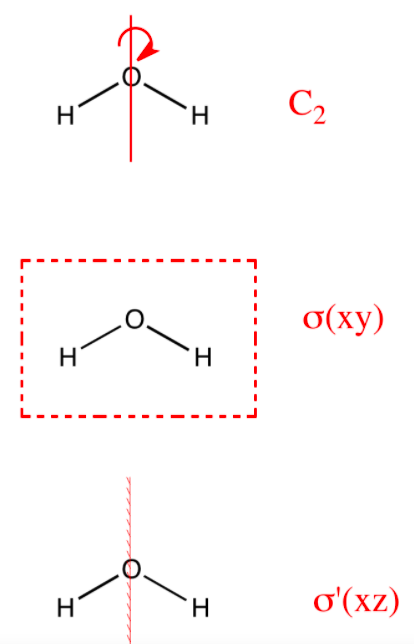
\includegraphics[width=.5\linewidth]{01.PNG}
        \caption{Molecular Orbital Energy Level Diagram for $H_2$}
        \label{fig:sub-first2}
\end{figure}



The overlap integral of the $H_2$ molecule: 
	 \begin{IEEEeqnarray}{rLl}
S=\int 1S_A(\vec{r})\cdot 1S_B(\vec{r})dr^3
	\end{IEEEeqnarray}
\tab Symmetry-adapted atomic orbitals: ($g$ is gerade, $u$ is ungerade)
	 \begin{IEEEeqnarray}{rLl}
\sigma_g &= (1S_A+1S_B)\cdot\frac{1}{\sqrt{2(1+S)}} \\
\sigma_u &= (1S_A-1S_B)\cdot\frac{1}{\sqrt{2(1-S)}} 
	\end{IEEEeqnarray}

\begin{figure}[H]
    \begin{subfigure}{.5\textwidth}
        \centering
        % 1
        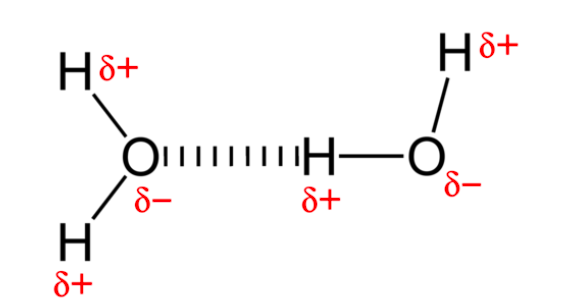
\includegraphics[width=.8\linewidth]{02.png}
        \caption{Bonding, $\sigma_g$ orbital}
        \label{fig:sub-first2}
    \end{subfigure}
    \begin{subfigure}{.5\textwidth}
        \centering
        % 2
        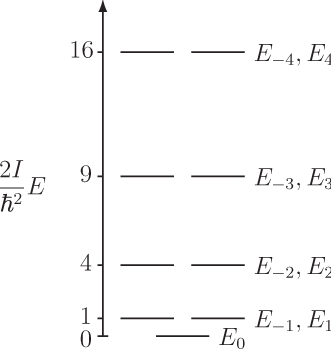
\includegraphics[width=.8\linewidth]{03.png}
        \caption{Anti-bonding, $\sigma_u$ orbital }
        \label{fig:sub-second2}
    \end{subfigure}
    \caption{$H_2$ Electronic Wavefunction}
    \label{fig:fig2}
\end{figure}

\subsubsection{Molecular Orbital Theory}
Here are some basic orbital diagram (after Hartree-Fock calculation usually). It introduces the the spin-up ($\alpha$) and spin-down ($\beta$) in molecular orbital diagram.
\begin{figure}[H]
        \centering
        % 1
        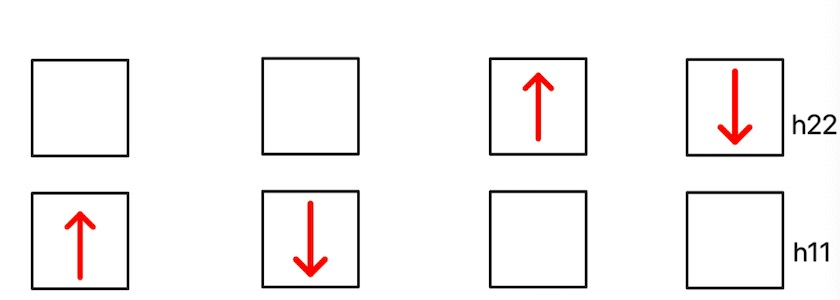
\includegraphics[width=.5\linewidth]{04.jpeg}
        \center{1($\sigma_g$)\tab \quad$\bar{1}$($\bar{\sigma}_g$)\tab\quad 2($\sigma_u$)\tab\quad$\bar{2}$($\bar{\sigma}_u$)}
        \caption{Molecular Orbital Diagram}
        \label{fig:sub-first2}
\end{figure}
\tab In molecular orbital theory, put both electrons in bonding orbital. The state is $|1\bar{1}\rangle$.

\subsubsection{Configuration Interaction}
True wavefunction for ground state in the minimal basis set is a linear combination.
	 \begin{IEEEeqnarray}{rLl}
|\psi_g\rangle &=c_1| \sigma_g \bar{\sigma}_g\rangle +c_2| \sigma_u \bar{\sigma}_u\rangle \notag  \\
&=c_1| 1\bar{1}\rangle +c_2| 2 \bar{2}\rangle
	\end{IEEEeqnarray}
\tab Note that the other determinants $\sigma_g\bar{\sigma}_u$ and  $\sigma_u\bar{\sigma}_g$ have wrong symmetry: $g \times u = u$.\\
\tab In CI : create Hamiltonian matrix $\langle \lambda|\hat{H}|\mu \rangle$
	
\begin{center}
\begin{tabular}{|c|c|c|} 
\hline 
$\hat{H}$ & $|1\bar{1}\rangle$ & $|2\bar{2}\rangle$ \\
\hline  
$\langle 1\bar{1}|$  & $\langle 1|\hat{h}|1\rangle + \langle \bar{1}|\hat{h}|\bar{1} \rangle +\langle 1\bar{1}||1\bar{1} \rangle $ & $\langle 1\bar{1}||2\bar{2} \rangle$\\
\hline  
$\langle 2\bar{2}|$  & $\langle 2\bar{2}||1\bar{1} \rangle$ & $\langle 2|\hat{h}|2\rangle + \langle \bar{2}|\hat{h}|\bar{2} \rangle +\langle 2\bar{2}||2\bar{2} \rangle $\\
\hline
\end{tabular}
\end{center}
\tab Simplify the matrix, we can get: $\left[ \begin{array}{cc}
    \varepsilon_1 & v \\ v & \varepsilon_2 \end{array} \right]$\\
\tab Next, diagonal the matrix in order to get the energy from the Hamiltonian matrix.
\begin{IEEEeqnarray}{rLl}
\left[ \begin{array}{cc}
    \varepsilon_1-\lambda & v \\ v & \varepsilon_2-\lambda \end{array} \right] \\
    (\varepsilon_1-\lambda )(\varepsilon_2-\lambda )-\nu^2 &=0 \\
    \varepsilon_1\varepsilon_2-\lambda(\varepsilon_1+\varepsilon_2)+\lambda^2-\nu^2 &=0 
	\end{IEEEeqnarray}
\tab We can get two solutions from this problem. 
\begin{itemize}
	\item Full CI solutions: 
\begin{IEEEeqnarray}{rLl}
\lambda &= \frac{1}{2}(\varepsilon_1+\varepsilon_2 \pm \sqrt{(\varepsilon_1+\varepsilon_2)^2-4 \left[ (\varepsilon_1-\varepsilon_2)-\nu^2\right]} ) \notag \\
&=  \frac{1}{2}(\varepsilon_1+\varepsilon_2) \pm \frac{1}{2}\sqrt{(\varepsilon_1-\varepsilon_2)^2+4\nu^2}
	\end{IEEEeqnarray}
	\item Second order perturbation(MP2) solutions: \\
	Approximation: 
\begin{IEEEeqnarray}{rLl}
\sqrt{(\varepsilon_1-\varepsilon_2)^2+4\nu^2} &= (\varepsilon_2-\varepsilon_1)\sqrt{1+\frac{4\nu^2}{(\varepsilon_2-\varepsilon_1 )^2}} \qquad\quad \text{use Taylor:}\sqrt{1+x}\approx 1+\frac{1}{2}x \\
&\approx (\varepsilon_1-\varepsilon_2)+\frac{1}{2}\frac{4\nu^2}{(\varepsilon_2-\varepsilon_1 )} \qquad\qquad \varepsilon_2-\varepsilon_1>0
	\end{IEEEeqnarray}
Energy with MP2 approximation: 
\begin{IEEEeqnarray}{rLl}
E_\pm \cong \frac{1}{2}(\varepsilon_1+\varepsilon_2 ) \pm\left[ \frac{1}{2}(\varepsilon_1-\varepsilon_2)+ \frac{\nu^2}{\varepsilon_2-\varepsilon_1 }\right]
	\end{IEEEeqnarray}
	Note that the lower energy, $E_-$, should be the energy of ground state; the higher energy, $E_+$, should be the energy of excited state.
\end{itemize}
\tab Sketch the potential energy curve (PES) for the $H_2$ molecule for variety of methods.
\begin{figure}[H]
        \centering
        % 1
        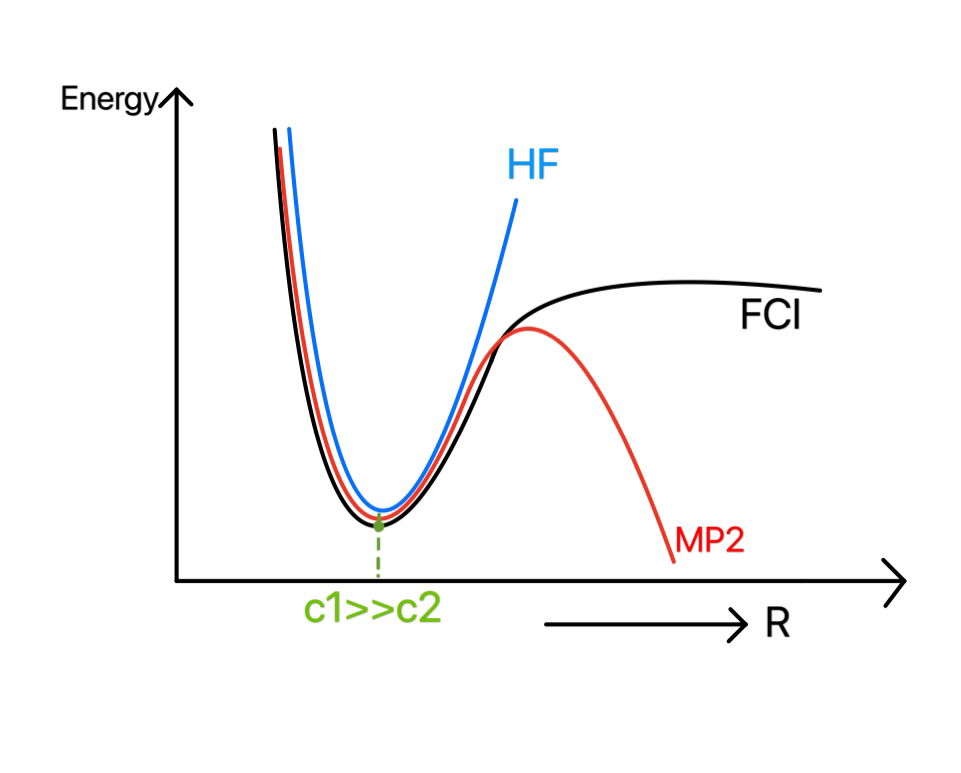
\includegraphics[width=.4\linewidth]{05.JPG}
        \caption{Potential Energy Curve at HF+ MP2 +FCI}
        \label{fig:sub-first2}
\end{figure}
Due to the FCI, the energy levels shift from $\varepsilon_1$ and $\varepsilon_2$. The shift depends on the $\hat{V}: \langle 1\bar{1}||2\bar{2} \rangle $, and $\varepsilon_1-\varepsilon_2$. The FCI (diagonalize the matrix) is the correct result at long distance. When $\varepsilon_1 \approx \varepsilon_2$, second order correction(MP2) is not accurate, because the existence of the term $\frac{\nu^2}{\varepsilon_1-\varepsilon_2}\rightarrow - \infty !$ This is the behaviour of MP2 in Gaussian.
	
	
\subsection{Example: Excited States of $H_2$ Molecule}
Let us analyze the excited states of $H_2$ molecule in a minimal basis, singlet $^1\Sigma_u$ and triplet $^3\Sigma_u$.
\begin{itemize}
	\item Triplet state: (both electrons are spin-up or spin-down in different orbitals)
\begin{figure}[H]
        \centering
        % 1
        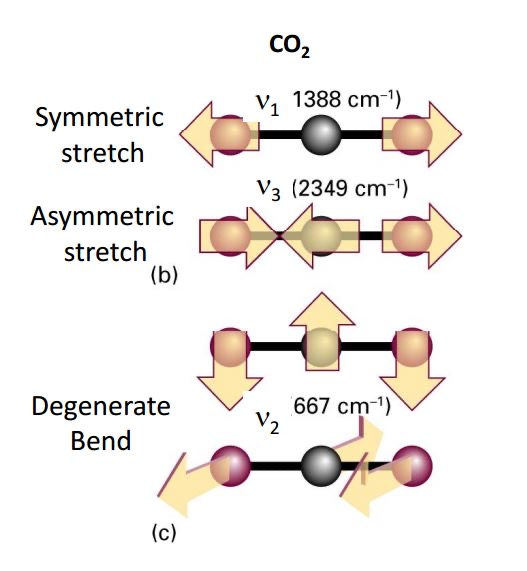
\includegraphics[width=.2\linewidth]{06.JPG}
        \caption{MO Diagram of Triplet States}
        \label{fig:sub-first2}
\end{figure}
\item Singlet or Triplet state: (linear combinations of spin-up electron and spin-down electron)
\begin{figure}[H]
        \centering
        % 1
        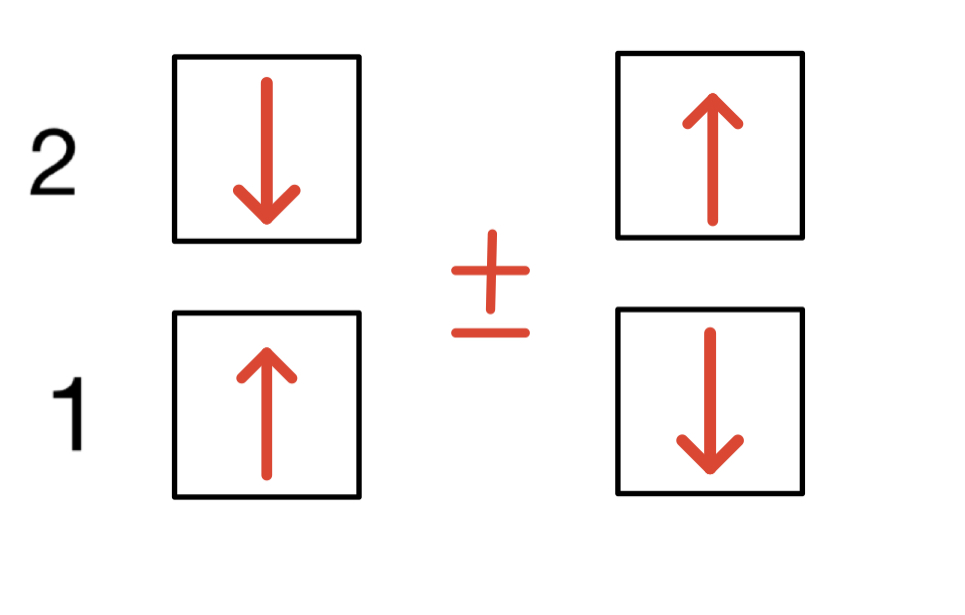
\includegraphics[width=.2\linewidth]{07.JPG}
        \caption{MO Diagram of Triplet States or Single States}
        \label{fig:sub-first2}
\end{figure}
\end{itemize}
\begin{IEEEeqnarray}{rLl}
E_T = \langle 1|\hat{h}|1\rangle +\langle 2|\hat{h}|2\rangle +\langle 12||12\rangle
	\end{IEEEeqnarray}
\tab To calculate singlet energy, set up the $2\times2$ matrix: 
\begin{center}
\begin{tabular}{|c|c|c|} 
\hline 
$\hat{H}$ & $|1\bar{2}\rangle$ & $|\bar{1}2\rangle$ \\
\hline  
$\langle 1\bar{2}|$  & $\langle 1|\hat{h}|1\rangle + \langle \bar{2}|\hat{h}|\bar{2} \rangle +\langle 1\bar{2}||1\bar{2} \rangle $ & $\langle 1\bar{2}||\bar{1}2 \rangle$\\
\hline  
$\langle \bar{1}2|$  & $\langle \bar{1}2||1\bar{2} \rangle$ & $\langle 2|\hat{h}|2\rangle + \langle \bar{1}|\hat{h}|\bar{1} \rangle +\langle \bar{1}2||\bar{1}2 \rangle $\\
\hline
\end{tabular}
\end{center}	
\tab What can we say about the integrals in terms of the spin-orbitals?\\
\tab Let us assume that the spatial parts of the orbitals are the same. $|1\rangle =\psi_1(\vec{r})|\alpha \rangle$,$|1\rangle =\psi_1(\vec{r})|\beta\rangle$.
\begin{IEEEeqnarray}{rLl}
\langle 1\bar{2}||1\bar{2}\rangle &= \langle 1\bar{2}|1\bar{2}\rangle -\langle 1\bar{2}|\bar{2}1\rangle \notag \\
&= \int \psi_1(1)\bar{\psi}_2(2) \frac{1}{r_{12}}\psi_1(1)\bar{\psi}_2(2) -\int \psi_1(1)\bar{\psi}_2(2) \frac{1}{r_{12}}\bar{\psi}_2(1)\psi_1(2) d1d2  \notag \\
&= \langle \alpha|\alpha \rangle_1 \langle\ \beta|\beta\rangle_2 -\langle \alpha|\beta \rangle_1 \langle\ \beta|\alpha \rangle_2 
	\end{IEEEeqnarray}
\tab NOTE:\\
\tab \tab The second integral is zero because the spin does note match. eg, $\langle \alpha(1)|\beta(1) \rangle=0 $\\
\tab On the other hand: 
\begin{IEEEeqnarray}{rLl}
\langle 1\bar{2}|| \bar{1} 2\rangle &= \langle 1\bar{2}|\bar{1}2\rangle -\langle 1\bar{2}|2\bar{1}\rangle \notag \\
&= 0 -  \langle 12|21 \rangle
	\end{IEEEeqnarray}	
\tab NOTE:\\
\tab \tab 1. The integral $\langle 12|21 \rangle$ is spatial integral.\\
\tab \tab 2. Because these integrals occur often, they get a special symbol for convenience. 
\begin{IEEEeqnarray}{rLl}
\langle ab|ab \rangle = J_{12} \quad &;\quad \langle 12|12 \rangle =J_{12} \\
\langle ab|ba \rangle = K_{12} \quad &;\quad \langle 12|21 \rangle =K_{12} \\
\langle a|\hat{h}|a \rangle =&\langle \bar{a}|\hat{h}| \bar{a} \rangle =h_{aa}
	\end{IEEEeqnarray}		
	\tab \tab \tab\tab $J$ is Coulomb integral; $K$ is Exchange integral.
	
	
	
Then, CI matrix can be reduced to: 
\begin{center}
\begin{tabular}{|c|c|c|} 
\hline 
$\hat{H}$ & $|1\bar{2}\rangle$ & $|\bar{1}2\rangle$ \\
\hline  
$\langle 1\bar{2}|$  & $h_{11}+ h_{22} +J_{12} $ & $-K_{12}$\\
\hline  
$\langle \bar{1}2|$  & $-K_{12}$ & $h_{11}+ h_{22} +J_{12} $\\
\hline
\end{tabular}
\end{center}	

\begin{IEEEeqnarray}{rLl}
\left[ \begin{array}{cc}
    \varepsilon & -K_{12} \\ -K_{12} & \varepsilon \end{array} \right]
    \left( \begin{array}{cc}
   1 \\ 1 \end{array} \right) &= ( \varepsilon- K_{12}) \left( \begin{array}{cc}
   1 \\ 1 \end{array} \right) \\
\left[ \begin{array}{cc}
    \varepsilon & -K_{12} \\ -K_{12} & \varepsilon \end{array} \right]
    \left( \begin{array}{cc}
   1 \\ -1 \end{array} \right) &= ( \varepsilon+ K_{12}) \left( \begin{array}{cc}
   1 \\ -1 \end{array} \right)   \\
   \notag \\
   E_-&= \varepsilon-K_{12} \\
   E_+&= \varepsilon+K_{12} 
	\end{IEEEeqnarray}		
\tab We can a higher energy, $E_+$, and a lower energy, $E_-$.\\
\tab Compare to triplet energy: 
\begin{IEEEeqnarray}{rLl}
h_{11}+ h_{12} + \langle 12||12\rangle &=h_{11}+ h_{12}+J_{12}-K_{12} \notag \\
&=\varepsilon -K_{12} \notag \\
&= E_- = E_{\text{triplet}}
	\end{IEEEeqnarray}		
\tab Similarly, the singlet energy:
\begin{IEEEeqnarray}{rLl}
 E_+ = E_{\text{singlet}}
	\end{IEEEeqnarray}	
\tab Like spin in Figure 5 is lower in energy than singlet coupled opposite spin (Figure 6).

\begin{itemize}
	\item The singlet spin(1 state): $\hat{S}_+ |12\rangle =|1\bar{2} \rangle -|\bar{1}2\rangle = |1\bar{2} \rangle +|\bar{1}2\rangle $
	\item The triplet spin(3 states): $\hat{S}_- |12\rangle =|12\rangle, |\bar{1}\bar{2}\rangle,|1\bar{2} \rangle +|\bar{1}2\rangle $
\end{itemize}
\tab The integral $K_{12}=\int\psi_1(1)\psi_2(2)\frac{1}{r_{12}}\psi_2(1)\psi_1(2)>0$, hence in this $2\times2$ model: $E_{\text{singlet}}>E_{\text{triplet}}$

This is the origin of Hund's rule in atomic spectra. Hund's rule: put the electrons(spin configuration) in the lowest energy. Because exchange interaction due to antisymmetry of wave function.







\subsection{Some Useful Notations for Evaluating Matrix Elements}
Using the Slater rules we can easily write down the energy expression for any determinant. \\
\tab Example: 
\begin{figure}[H]
        \centering
        % 1
        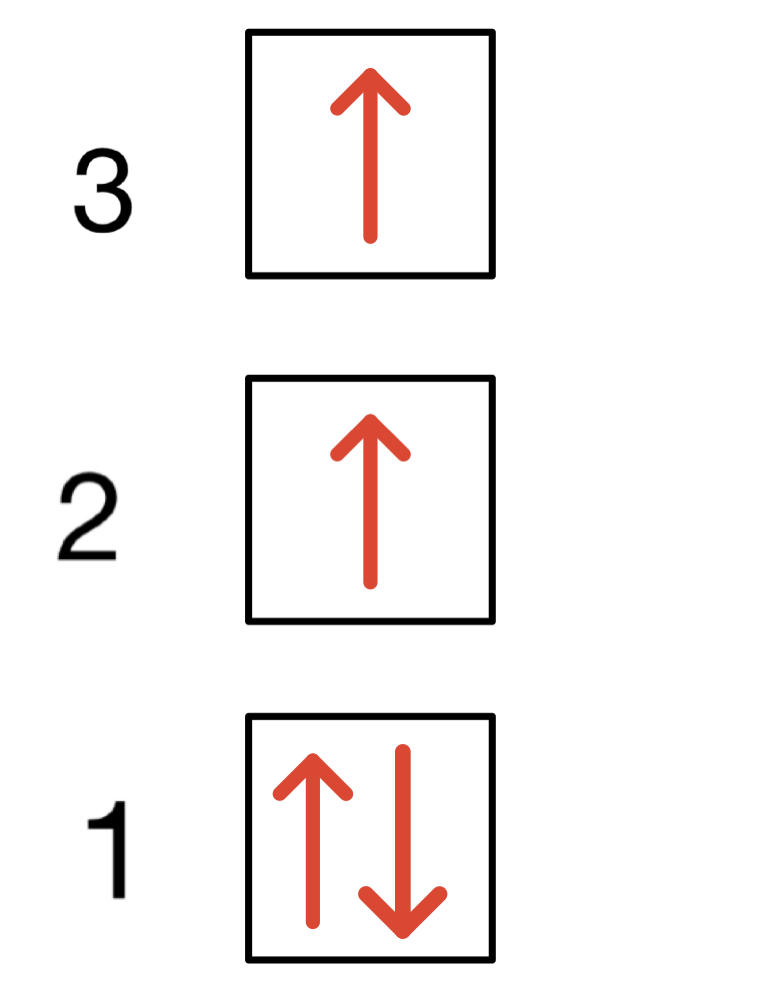
\includegraphics[width=.15\linewidth]{08.JPG}
        \caption{MO Diagram of Example}
        \label{fig:sub-first2}
\end{figure}
The element of Slater rules are the diagonal elements, $\langle K|\hat{H}|K\rangle$. The energy of this determinant: 
\begin{IEEEeqnarray}{rLl}
E &= \langle 1|\hat{h}|1\rangle + \langle \bar{1}|\hat{h}|\bar{1}\rangle +\langle 2|\hat{h}|2\rangle+\langle 3|\hat{h}|3\rangle \notag \\
&+\langle 1\bar{1}||1\bar{1}\rangle+\langle 12||12\rangle+\langle 13||13\rangle+\langle  \bar{1}2||\bar{1}2\rangle+\langle  \bar{1}2||\bar{1}3\rangle+\langle 23||23\rangle
	\end{IEEEeqnarray}	

Here is the general formula of energy:
\begin{IEEEeqnarray}{rLl}
E &= \sum_{a \in K}\langle a|\hat{h}|a\rangle +\sum_{a<b\in K}\langle ab||ab\rangle
	\end{IEEEeqnarray}	


Let us condense a little bit and consider spin explicitly. Assume same spatial orbitals for $\alpha$ and $\beta$ spin. Consider real orbitals only.
\begin{IEEEeqnarray}{rLl}
\langle a|\hat{h}|a\rangle &=\langle \bar{a}|\hat{h}|\bar{a} \rangle =h_{aa} \\
\langle a|\hat{h}|\bar{b} \rangle &= 0 \\
\langle ab|ab \rangle &=J_{ab} \\
\langle ab|ba \rangle &=K_{ab}
	\end{IEEEeqnarray}	
	\tab NOTE:
	\begin{itemize}
		\item $J_{ab}$ is spatial Colomb integral. Coulomb interaction between $|\psi_a(1)|^2$ and $|\psi_b(2)|^2$
		\begin{IEEEeqnarray}{rLl}
J_{ab}=  \int \psi_a^*(1)\psi_a(1) \frac{1}{r_{12}}\psi_b^*(2)\psi_b(2)d1d2
	\end{IEEEeqnarray}
		\item $K_{ab}$ is spatial exchange integral. Exchange interaction between $\psi_a(1)\psi_b(1)$ and $\psi_a(2)\psi_b(2)$. $\psi_a\psi_b$ may not be positive everywhere, but $K_{ab}>0$ is always true. 
	\begin{IEEEeqnarray}{rLl}
K_{ab}=  \int \psi_a^*(1)\psi_b(1) \frac{1}{r_{12}}\psi_a^*(2)\psi_b(2)d1d2
	\end{IEEEeqnarray}
	\end{itemize}

We would have more integrals $\langle pq|rs \rangle$, but in the example we can use the 'diagonal' integrals exclusively.
	\begin{IEEEeqnarray}{rLl}
\langle ab||ab \rangle   = \langle ab|ab \rangle -\langle ab|ba \rangle &=J_{ab}-K_{ab} \\
\langle a \bar{b}||a\bar{b} \rangle =\langle a \bar{b}|a\bar{b} \rangle - \langle a \bar{b}|\bar{b}a \rangle &= J_{ab} \\
\langle a \bar{b}||\bar{a}b \rangle =-\langle a \bar{b}|b \bar{a} \rangle =-K_{ab}
	\end{IEEEeqnarray}
\tab Moreover the integrals/ orbitals are real. Then, we can flip(interchange) the a and b labels due to symmetry.
	\begin{IEEEeqnarray}{rLl}
\langle aa|bb \rangle   = \langle ab|ba \rangle = K_{ab} \\
\langle a \bar{a}||b\bar{b} \rangle =\langle a \bar{a}|b\bar{b} \rangle -\cancelto{0}{\langle a \bar{a}|\bar{b}b \rangle} =K_{ab}
	\end{IEEEeqnarray}
\tab Using these integrals we can set up some interesting problems.

\subsection{Example: Carbon Atom}
Example: Carbon.\\
\tab Firstly, we need some background about angular momentum. 
See Link:  \href{http://scienide2.uwaterloo.ca/~nooijen/website_new_20_10_2011/Chem440_quantum/Many_electron_angular_momentum.pdf}{Atomic Term Symbol}.
\begin{itemize}
	\item  Angular momentum theory: \\
 For states, we use upper case.\\
 The orbital angular momentum: $L, M_L=-L,\ldots,+L$. $(2L+1)$ states associated with orbital.\\
 The spin angular momentum: $S, M_S=-S,\ldots,+S$. $(2S+1)$ states associated with spin.
 \item The easiest way to construct: 
 \begin{itemize}
 \item[1)] highest $M_S $: \tab   $M_S = \sum m_s$\\
 \tab\tab\tab\tab $m_s=\frac{1}{2}$ for $\alpha$ \tab\tab $m_s=-\frac{1}{2}$ for $\beta$
 \item[2)] highest $M_L $: \tab   $M_L = \sum m_l$\\


 
 \end{itemize}
 \item Term symbol: $^{(2S+1)}L$\\
 $L= 0,1,2,3,4 \Rightarrow S,P,D,F,G $\\
 
\end{itemize}




Return to atom: Carbon.\\
\tab The ground state configuration of Carbon atom: $1s^22s^2(2p)^2$. There are $C_6^2 =$15 different quantum states.\\
\tab Regardless of the close shell ($1s^22s^2$), we have six spin-orbitals, $p_1,p_0,p_{-1}, \bar{p}_1,\bar{p}_0,\bar{p}_{-1}$. 

\begin{itemize}
	\item [1)] Highest $M_S$, of theses highest $M_L$: $|p_1p_0|$ state \\
	$M_S =\frac{1}{2}+\frac{1}{2}=1 \tab\tab S=M_S=1 \tab\tab (2S+1)=3$\\
	$ M_L= 1+0=1  \tab\tab L=M_L=1 \tab\tab (2L+1)=3$\\
	There are 9 degeneracies in total. $(2S+1)(2L+1)=9$.\\
	Term symbol $^3P$ has 9 states. (Neglect $J-$coupling spin-orbital.)\\
	These 9 states are all degenerate.
	\item [2)] Highest $M_L$, of theses highest $M_S$: $|p_1\bar{p}_1|$ state
	\\
	$M_S =\frac{1}{2}-\frac{1}{2}=0 \tab\tab S=M_S=0 \tab\tab (2S+1)=1$\\
	$ M_L= 1+1=2  \tab\tab L=M_L=2 \tab\tab (2L+1)=5$\\
	There are 9 degeneracies in total. $(2S+1)(2L+1)=5$.\\
	Term symbol $^1D$ has 5 states. (Neglect $J-$coupling spin-orbital.)\\
	These 5 states are all degenerate.
	\item [3)] One state left: $^1S$
\end{itemize}
\tab We get degeneracy pattern from angular momentum theory.

Next, we will do Carbon atom by diagonalizing Hamiltonian $15 \times 15$ matrix. Use symmetry to do small blocks. We will use abbreviate symbols, $x,y,z,\bar{x},\bar{y},\bar{z}$, represent real orbitals $p_x,p_y,p_z, \bar{p}_x,\bar{p}_y,\bar{p}_z$. There are three types of $M_S$ function: 
\begin{itemize}
	\item $M_S=0$: $|x\bar{x}|, |y\bar{y}|, |z\bar{z}|, \\ \tab \tab |x\bar{y}|, |x\bar{z}|, |y\bar{x}|, |y\bar{z}|,|z\bar{x}|, |z\bar{y}|$
	\item $M_S=1$: $|xy|, |xz|, |yz|$
	\item $M_S=-1$: $|\bar{x}\bar{y}|,|\bar{x}\bar{z}|, |\bar{y}\bar{z}|$
\end{itemize}
 Types of 2-electron integrals: 
\begin{itemize}
	\item[1)] $h_{xx}=h_{yy}=h_{zz}\equiv h$
	\item[2)] $\langle xx|xx \rangle = \langle yy|yy\rangle =\langle zz|zz\rangle =D $
	\item[3)] $\langle xy|xy \rangle = \langle xz|xz\rangle =\langle yz|yz\rangle =J $
	\item[4)] $\langle xy|yx \rangle = \langle xz|zx\rangle =\langle yz|zy\rangle = \langle xx|yy \rangle = \langle xx|zz\rangle =\langle yy|zz\rangle =K$ 
	\item[5)] Integrals in which $x,y,z$ occur an odd number of times are zero. 
	\item[6)] There is one more important about relation between the integrals:  $D=J+2K$
	
\end{itemize}

Now we can partition Hamiltonian in small sub-blocks:
\begin{itemize}
	\item $M_S=1$: 
	\begin{center}
\begin{tabular}{|c|c|c|c|} 
\hline 
 & $xy$ & $xz$ & $yz$\\
\hline  
$xy$ & $2h+J-K$ & 0 & 0\\
\hline  
$xz$  & 0 & $2h+J-K$ & 0\\
\hline  
$yz$  & 0 &0 & $2h+J-K$\\
\hline
\end{tabular}
\end{center}
 $E(^3P)= 2h+J-K$, same for $M_S= -1$, likewise $\bar{x}\bar{y},\bar{x}\bar{z}, \bar{y}\bar{z}$
 \item $M_S=0$: 
 	\begin{center}
\begin{tabular}{|c|c|c|} 
\hline 
 & $x\bar{y}$ & $y\bar{x}$ \\
\hline  
$x\bar{y}$ & $2h+J$ & $+K$\\
\hline  
 $y\bar{x}$ & $+K$ & $2h+J$\\
\hline
\end{tabular}
\\ \hspace*{\fill} \\
NOTE: $\langle x\bar{y}||y\bar{x} \rangle =\langle x\bar{y}|y\bar{x} \rangle - \langle x\bar{y}|\bar{x}y \rangle = \langle xy|yx \rangle -0 = K $
\end{center}
 $E= 2h+J \pm K$,  for $x\bar{y}+\bar{x}y$\\
 $E(^3P)= 2h+J-K$,  for $|x\bar{y}\rangle -|y\bar{x}\rangle$\\
 $E(^1D)= 2h+J+K$,  for $|x\bar{y}\rangle +|y\bar{x}\rangle$\\
Same for $x\bar{z}\pm z\bar{x}$ and $y\bar{z}\pm z\bar{y}$ 
 
$\Rightarrow$ 9 states found for triplet $^3P$ ; 3 states for singlet $^1D$.
 
 
Finally: 
	\begin{center}
\begin{tabular}{|c|c|c|c|} 
\hline 
 & $x\bar{x}$ & $y\bar{y}$  &$z\bar{z}$\\
\hline  
$x\bar{x}$ & $2h+D$ & $K$ & $K$\\
\hline  
$y\bar{y}$  & $K$ &$2h+D$ & $K$\\
\hline  
$z\bar{z}$ & $K$ & $K$ & $2h+D$\\
\hline
\end{tabular}
\\ \hspace*{\fill} \\
NOTE: $\langle x\bar{x}||y\bar{y} \rangle =\langle x\bar{y}|y\bar{x} \rangle = K $
\end{center}
Familiar with Hamiltonian, diagonalize the matrix and get eigenvectors and eigenvalues.\\
The eigenvector $\left( \begin{array}{ccc}
   1 \\ 1 \\1 \end{array} \right)$ with the eigenvalue $E= 1h+D+2K =2h+J+4K \Rightarrow$  $^1S$ .\\
The eigenvectors $\left( \begin{array}{ccc}
   0 \\ 1 \\-1 \end{array} \right)$ and $\left( \begin{array}{ccc}
   2 \\ -1 \\-1 \end{array} \right)$ with the same eigenvalue $E= 2h+D-K =2h+J+K \Rightarrow$  $^1D$ .\\   
 Hence, $^1S =|x\bar{x}\rangle+|y\bar{y}\rangle+|z\bar{z}\rangle$
 \\ \hspace*{\fill} \\
 \tab\quad  $^1D = \left\{ \begin{aligned}
       |y\bar{y}\rangle - |z\bar{z}\rangle \\ 2|x\bar{x}\rangle-|y\bar{y}\rangle-|z\bar{z}\rangle 
       \end{aligned}\right.$\\
 \tab\quad  $^1D = \left\{ \begin{aligned}
       |x\bar{x}\rangle - |y\bar{y}\rangle \\ 2|z\bar{z}\rangle-|x\bar{x}\rangle-|y\bar{y}\rangle 
       \end{aligned}\right.$
\end{itemize}



Atom: small but complicated due to degeneracies and small excitation energies. Many states are linear combinations of determinants. \\
\tab Hartree-Fock is useless, because HF method depends on single determinants.\\
\tab DFT is also useless. \\
\tab Electronic structure (multireference method): Qualitative wave functions, required more than one determinants.






























\end{document}